\documentclass[aspectratio=169,dvipsnames]{beamer}
\usetheme{Pittsburgh}
\usepackage[utf8]{inputenc}
\usepackage{amsmath}
\usepackage{amsfonts}
\usepackage{amssymb}
\usepackage{graphicx}
\usepackage{multicol}
\usepackage{wrapfig}
\usepackage{hyperref}
\usepackage{tikz}
\usepackage{censor}

\usetikzlibrary{shapes,arrows,chains}

\author{Jonas Betzendahl}
\title{Digital Self-Defense}

\beamertemplatenavigationsymbolsempty 
\setbeamertemplate{footline}[frame number]

%src: https://tex.stackexchange.com/questions/34921/how-to-overlap-images-in-a-beamer-slide
\def\Put(#1,#2)#3{\leavevmode\makebox(0,0){\put(#1,#2){#3}}}

%https://tex.stackexchange.com/questions/70448/dont-count-backup-slides
\newcommand{\backupbegin}{
   \newcounter{finalframe}
   \setcounter{finalframe}{\value{framenumber}}
}
\newcommand{\backupend}{
   \setcounter{framenumber}{\value{finalframe}}
}

\begin{document}

%------------------------------------------------------------------------------------
\section{Introduction}

\begin{frame}
\begin{center}
\vfill
\huge Digital Self-Defense
\normalsize 
\smallskip
\smallskip

Levelling up your defense in a world\\ that is levelling up its offense.
\bigskip\bigskip

\large Jonas Betzendahl, M.Sc.\\
2019 -- 12 -- 06
\bigskip\bigskip

\href{https://twitter.com/lambdatotoro}{
\includegraphics[scale=0.125]{images/twitter_logo.png}}
\href{https://chaos.social/@lambdatotoro}{\includegraphics[scale=0.125]{images/mastodon_logo.png}}
\href{https://github.com/lambdaTotoro}{
\includegraphics[scale=0.125]{images/github_logo.png}}
\href{https://whispeer.de/en/user/jbetzend}{
\includegraphics[scale=0.125]{images/whispeer_logo.png}}

\texttt{@lambdaTotoro (@chaos.social)}
\end{center}
\end{frame}

\begin{frame}
\frametitle{Who am I?}
\end{frame}

\begin{frame}
\frametitle{Who are you?}
\end{frame}

\begin{frame}
\frametitle{What is the problem?}
\end{frame}

\begin{frame}
\frametitle{What is \emph{not} the solution?}
Don't take nudes, don't be online, never do anything convenient.
\end{frame}

\begin{frame}
\frametitle{What \emph{is} the solution?}
Be aware, be informed.
\end{frame}

\begin{frame}
\frametitle{What is this workshop?}
Please ask questions immediately
\end{frame}

%------------------------------------------------------------------------------------

\section{Technical Attacks}
\begin{frame}
\begin{center}
\huge Technical Attacks\normalsize
\end{center}
\end{frame}

\subsection{Passwords}

\subsubsection{Secure Passwords}

\begin{frame}
\frametitle{Secure Passwords}
\end{frame}

\begin{frame}
\frametitle{Secure Passwords}
\end{frame}

\subsubsection{Password Managers}

\begin{frame}
\frametitle{Password Managers}
\end{frame}

\subsubsection{Security Questions}

\begin{frame}
\frametitle{Security Questions}
\end{frame}


\subsubsection{Phone Security}

\setbeamercolor{background canvas}{bg=Apricot}

\begin{frame}
\frametitle{Smartphone Security (Quiz)}

Which of these is the safest way of locking your phone?
\medskip

\begin{itemize}
\item A six-digit PIN
\item A six-point swipe pattern
\item Your fingerprint / face as a biometric pattern
\end{itemize}

\end{frame}

\begin{frame}
\frametitle{Smartphone Security (Quiz)}

Which of these is the safest way of locking your phone?
\medskip

\begin{itemize}
\item \textcolor{ForestGreen}{A six-digit PIN}
\item \textcolor{Red}{A six-point swipe pattern}
\item \textcolor{Red}{Your fingerprint / face as a biometric pattern}
\end{itemize}

\end{frame}

\setbeamercolor{background canvas}{bg=white}

\begin{frame}
\frametitle{Swipe Patterns}

\begin{minipage}{0.5\textwidth}
foo
\end{minipage}%
\begin{minipage}{0.5\textwidth}
\begin{center}

\includegraphics[scale=0.3]{images/swipe_unlock.jpg} 
\end{center}
\end{minipage}

\end{frame}

\begin{frame}
\frametitle{Biometrics}

\begin{minipage}{0.5\textwidth}
\begin{center}
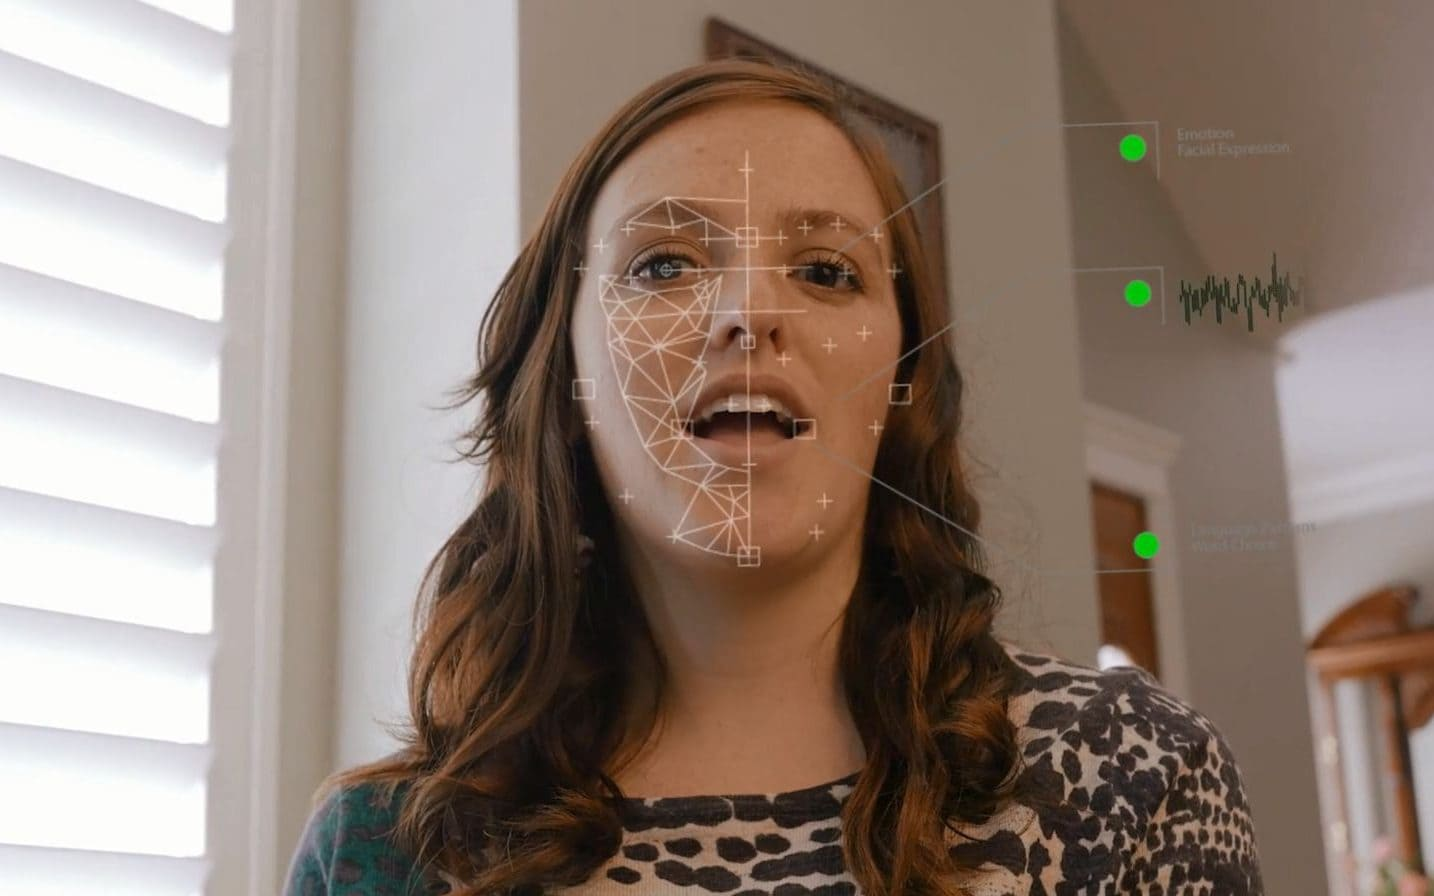
\includegraphics[width=0.95\textwidth, keepaspectratio]{images/hirevue.jpeg}
\end{center}
\end{minipage}\pause\quad
\begin{minipage}{0.45\textwidth}
Biometrics (such as fingerprints, facial recognition, \dots) are very convenient!
\pause\medskip

But they are not good passwords! For example, they can't be \dots

\begin{itemize}
\pause\item changed or reset,
\pause\item ``forgotten'',
\pause\item fake-proofed
\end{itemize}
\end{minipage}

\pause\bigskip
\begin{center}
\Large
Biometrics are better thought of as \emph{user names}, not \emph{passwords}!
\end{center}
\end{frame}

\subsection{Malware}

\subsubsection{Keyloggers, Trojans, Viruses}

\begin{frame}
\frametitle{Keyloggers, Trojans, Viruses}
\end{frame}

\subsubsection{Stalkerware}

\begin{frame}
\frametitle{Stalker- \& Spouseware}
\end{frame}

\begin{frame}
\frametitle{How to spot stalkerware}
\end{frame}

\subsubsection{Anti-virus Software}

\begin{frame}
\frametitle{Anti-Virus}
\end{frame}

\begin{frame}
\frametitle{Not just for Desktops}
\end{frame}

\subsection{VPNs}

\begin{frame}
\frametitle{VPNs}
\end{frame}

\begin{frame}
\frametitle{VPN Advertisement Claims:}

\begin{itemize}
\item \textbf{``Everytime you connect to public Wi-Fi, you risk data theft!''}
\pause \item \textbf{``This VPN uses military-grade encryption!''}\\
True, but meaningless.
\end{itemize}


\pause
\begin{center}
\emph{Recommended Watch: Tom Scott's ``This Video Is Sponsored By \censor{Nord}VPN''}
\end{center}
\end{frame}

%------------------------------------------------------------------------------------

\section{Social Attacks}
\begin{frame}
\begin{center}
\huge Social Attacks
\end{center}
\end{frame}

\begin{frame}
\frametitle{How it works\dots}
\begin{minipage}[t]{0.49\textwidth}
\begin{center}
\vspace*{-15pt}
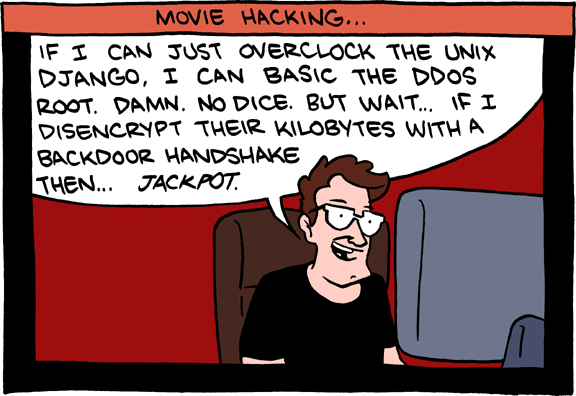
\includegraphics[width=\textwidth,keepaspectratio]{images/hackerman-1}
\end{center}
\end{minipage}
\begin{minipage}[t]{0.49\textwidth}
\begin{center}
\vspace*{15pt}
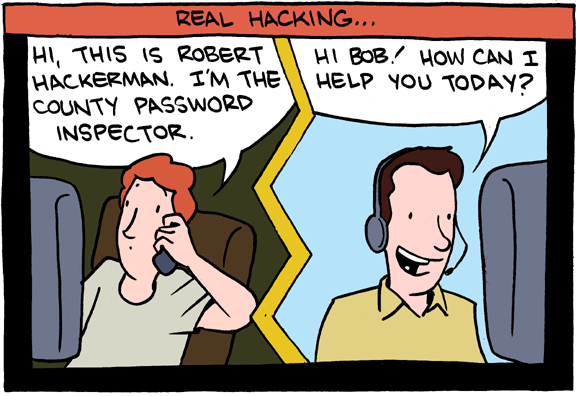
\includegraphics[width=\textwidth,keepaspectratio]{images/hackerman-2}
\end{center}
\end{minipage}
\end{frame}

\subsection{Phishing}

\subsection{Social Engineering}

%------------------------------------------------------------------------------------

\section{Miscellaneous}
\begin{frame}
\begin{center}
\huge Miscellaneous
\end{center}
\end{frame}

\subsection{Fake News}

\begin{frame}
\frametitle{Fake News (1)}
\end{frame}

\setbeamercolor{background canvas}{bg=Apricot}

\begin{frame}
\frametitle{Fake News (Quiz)}
\end{frame}

\setbeamercolor{background canvas}{bg=white}


%------------------------------------------------------------------------------------

\section{Conclusion}
\begin{frame}
\begin{center}
\huge Conclusion
\end{center}
\end{frame}

\begin{frame}
\frametitle{Recap}
\end{frame}

\begin{frame}
\frametitle{Things you can do this weekend:}
\begin{itemize}
\pause\item\textbf{\dots install/change lockscreen PIN.}
\pause\item\textbf{\dots get a password manager.}
\pause\item\textbf{\dots get a secure (end-to-end) messenger.}
\pause\item\textbf{\dots review apps \& permissions on your phone.}
\pause\item\textbf{\dots install anti-virus software.}\\
\emph{Especially} on your phone. 
\pause\item\textbf{\dots enable 2FA where applicable.}
\end{itemize}
\end{frame}

\begin{frame}
\frametitle{Final Thoughts}
\end{frame}

%------------------------------------------------------------------------------------
\appendix
\backupbegin

\section{End}

\begin{frame}
\frametitle{Resources}

\begin{itemize}
\item \emph{Surveillance Self-Defense} @ EFF, \url{https://ssd.eff.org}
\item \emph{Coalition against Stalkerware}, \url{https://stopstalkerware.org/}
\end{itemize}

\end{frame}

\begin{frame}
\frametitle{Sources}
\footnotesize

\begin{itemize}
\item Wired, \emph{Don't Rely On an Unlock Pattern To Secure Your Android Phone}: \\
\url{https://www.wired.com/story/android-unlock-pattern-or-pin/}
\item UK Advertisement Regulatory Ruling Re: NordVPN:\\
\url{https://www.asa.org.uk/rulings/tefincom-sa-a19-547668.html}
\item Tom Scott's ``This Video Is Sponsored By \censor{Nord}VPN'':\\
\url{https://www.youtube.com/watch?v=WVDQEoe6ZWY}
\item\dots
\end{itemize}

\end{frame}

\backupend
\end{document}

